% Practice Test 23 — Texas Edition
% Questions: 30 (15 MC + 15 SA)
% Generated by scripts/generate_practice_tests.py

\begin{practiceQuestion}{1-3-q05}{mc}
\begin{questionText}
A car travels at a constant speed. It goes $150$ miles in $2.5$ hours. What is the constant of proportionality?
\end{questionText}
\choiceA{$30$ mph}
\choiceB{$60$ mph}
\choiceC{$75$ mph}
\choiceD{$150$ mph}
\correctAnswer{B}
\explanation{$k = \frac{150}{2.5} = 60$ miles per hour.}
\end{practiceQuestion}

\begin{practiceQuestion}{1-6-q30}{gsa}
\begin{questionText}
The table shows how many batches of muffins a bakery can make and the total flour used. How many cups of flour are needed for $15$ batches?

\begin{center}
\begin{tabular}{|c|c|}
\hline
\textbf{Batches} & \textbf{Flour (cups)} \\ \hline
$3$ & $7\frac{1}{2}$ \\ \hline
$6$ & $15$ \\ \hline
$9$ & $22\frac{1}{2}$ \\ \hline
$15$ & $?$ \\ \hline
\end{tabular}
\end{center}
\end{questionText}
\correctAnswer{$37\frac{1}{2}$ cups}
\explanation{$k = \frac{7.5}{3} = 2.5$ cups per batch. For $15$ batches: $2.5 \times 15 = 37.5 = 37\frac{1}{2}$ cups.}
\end{practiceQuestion}

\begin{practiceQuestion}{2-1-q21}{sa}
\begin{questionText}
$56$ is $80\%$ of what number?
\end{questionText}
\correctAnswer{$70$}
\explanation{Divide: $56 \div 0.80 = 70$.}
\end{practiceQuestion}

\begin{practiceQuestion}{2-3-q14}{mc}
\begin{questionText}
A gym membership increased from $\$45$ per month to $\$54$ per month. What is the percent increase?


\numberLine[1]{45}{55}
\end{questionText}
\choiceA{$9\%$}
\choiceB{$15\%$}
\choiceC{$18\%$}
\choiceD{$20\%$}
\correctAnswer{D}
\explanation{Change: $54 - 45 = 9$. Percent increase: $9 \div 45 = 0.20 = 20\%$.}
\end{practiceQuestion}

\begin{practiceQuestion}{2-6-q22}{sa}
\begin{questionText}
You earned $\$180$ in interest on $\$2{,}000$ over $3$ years. What was the interest rate?
\end{questionText}
\correctAnswer{$3\%$}
\explanation{$180 = 2{,}000 \times r \times 3$ → $180 = 6{,}000r$ → $r = 0.03 = 3\%$.}
\end{practiceQuestion}

\begin{practiceQuestion}{2-8-q28}{gmc}
\begin{questionText}
The bar graph shows interest earned on a $\$1{,}000$ deposit at three different banks after $1$ year. Which bank pays the highest interest rate?

\begin{center}
\begin{tikzpicture}[scale=0.7]
  \draw[thick,->] (0,0) -- (0,5) node[above] {Interest (\$)};
  \draw[thick,->] (0,0) -- (8,0);
  \foreach \y/\label in {0/0, 1/10, 2/20, 3/30, 4/40} {
    \draw (-0.1,\y) -- (0.1,\y);
    \node[left] at (-0.15,\y) {\footnotesize \$\label};
  }
  % Bank X
  \fill[funBlue!70] (0.5,0) rectangle (2,2);
  \node[below] at (1.25,0) {\footnotesize Bank X};
  \node[above] at (1.25,2) {\footnotesize \$20};
  % Bank Y
  \fill[funRed!70] (3,0) rectangle (4.5,3.5);
  \node[below] at (3.75,0) {\footnotesize Bank Y};
  \node[above] at (3.75,3.5) {\footnotesize \$35};
  % Bank Z
  \fill[green!50!black] (5.5,0) rectangle (7,1.5);
  \node[below] at (6.25,0) {\footnotesize Bank Z};
  \node[above] at (6.25,1.5) {\footnotesize \$15};
\end{tikzpicture}
\end{center}
\end{questionText}
\choiceA{Bank X}
\choiceB{Bank Y}
\choiceC{Bank Z}
\choiceD{They all pay the same}
\correctAnswer{B}
\explanation{Bank Y earned $\$35$ on $\$1{,}000$, which is $3.5\%$ — the highest of the three.}
\end{practiceQuestion}

\begin{practiceQuestion}{2-9-q15}{mc}
\begin{questionText}
A student earns $\$200$ per month from a part-time job. She spends $\$60$ on a phone plan (fixed) and $\$80$ on food (variable). How much can she save?
\end{questionText}
\choiceA{$\$140$}
\choiceB{$\$60$}
\choiceC{$\$80$}
\choiceD{$\$120$}
\correctAnswer{B}
\explanation{$200 - 60 - 80 = \$60$ available to save.}
\end{practiceQuestion}

\begin{practiceQuestion}{2-10-q13}{mc}
\begin{questionText}
In the formula $A = P(1 + r)^t$, what does $t$ represent?
\end{questionText}
\choiceA{Tax rate}
\choiceB{Total amount}
\choiceC{Number of years}
\choiceD{Type of account}
\correctAnswer{C}
\explanation{$t$ is the number of years the money is invested or borrowed.}
\end{practiceQuestion}

\begin{practiceQuestion}{4-1-q08}{mc}
\begin{questionText}
Evaluate $-4y + 10$ when $y = 3$.
\end{questionText}
\choiceA{$22$}
\choiceB{$-2$}
\choiceC{$2$}
\choiceD{$-22$}
\correctAnswer{B}
\explanation{Substitute: $-4(3) + 10 = -12 + 10 = -2$.}
\end{practiceQuestion}

\begin{practiceQuestion}{4-2-q25}{sa}
\begin{questionText}
Write an expression with three terms that simplifies to $4n + 7$.
\end{questionText}
\correctAnswer{Answers vary, e.g., $n + 3n + 7$ or $5n - n + 7$}
\explanation{Any expression whose like terms combine to give $4n + 7$ is correct. For example: $n + 3n + 7 = 4n + 7$.}
\end{practiceQuestion}

\begin{practiceQuestion}{5-3-q27}{gmc}
\begin{questionText}
The diagram shows two equal groups. Which equation represents this, and what is $x$?

\begin{center}
\begin{tikzpicture}[scale=0.6]
  % Group 1
  \draw[thick,fill=funBlue!20,rounded corners] (-0.5,-0.5) rectangle (3.5,2.5);
  \node[draw,fill=funBlue!40,minimum size=0.6cm] at (0.5,1.5) {$x$};
  \node at (1.5,1.5) {$+$};
  \node[draw,fill=funOrange!40,minimum size=0.6cm] at (2.5,1.5) {$4$};
  \node at (1.5,0.2) {Group 1};
  % Group 2
  \draw[thick,fill=funBlue!20,rounded corners] (5,-0.5) rectangle (9,2.5);
  \node[draw,fill=funBlue!40,minimum size=0.6cm] at (6,1.5) {$x$};
  \node at (7,1.5) {$+$};
  \node[draw,fill=funOrange!40,minimum size=0.6cm] at (8,1.5) {$4$};
  \node at (7,0.2) {Group 2};
  % Total
  \draw[decorate,decoration={brace,amplitude=8pt}] (9.2,2.7) -- (9.2,-0.7);
  \node[right] at (9.5,1) {$= 22$};
\end{tikzpicture}
\end{center}
\end{questionText}
\choiceA{$2(x + 4) = 22$, $x = 7$}
\choiceB{$2x + 4 = 22$, $x = 9$}
\choiceC{$x + 8 = 22$, $x = 14$}
\choiceD{$2(x + 4) = 22$, $x = 3$}
\correctAnswer{A}
\explanation{Two identical groups of $(x + 4)$: $2(x + 4) = 22$. Divide by $2$: $x + 4 = 11$. Subtract $4$: $x = 7$.}
\end{practiceQuestion}

\begin{practiceQuestion}{5-4-q10}{mc}
\begin{questionText}
Solve $\dfrac{x}{6} - \dfrac{2}{3} = \dfrac{1}{2}$.
\end{questionText}
\choiceA{$x = 3$}
\choiceB{$x = 7$}
\choiceC{$x = -1$}
\choiceD{$x = 10$}
\correctAnswer{B}
\explanation{Multiply every term by $6$: $x - 4 = 3$. Add $4$: $x = 7$. Check: $\frac{7}{6} - \frac{2}{3} = \frac{7}{6} - \frac{4}{6} = \frac{3}{6} = \frac{1}{2}$ \checkmark.}
\end{practiceQuestion}

\begin{practiceQuestion}{5-5-q24}{sa}
\begin{questionText}
Solve $\dfrac{x}{2} + 7 \leq 12$.
\end{questionText}
\correctAnswer{$x \leq 10$}
\explanation{Subtract $7$: $\frac{x}{2} \leq 5$. Multiply by $2$: $x \leq 10$.}
\end{practiceQuestion}

\begin{practiceQuestion}{5-6-q30}{gsa}
\begin{questionText}
A student has test scores of $78$, $85$, and $90$. She needs an average of at least $85$ on four tests to earn an A. Solve the inequality to find the minimum score $s$ on the fourth test, and describe the graph.

\begin{center}
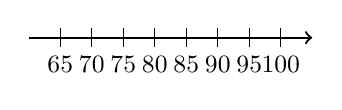
\begin{tikzpicture}[scale=0.08]
  \draw[thick,->] (60,0) -- (105,0);
  \foreach \x in {65,70,...,100} {
    \draw (\x,1.5) -- (\x,-1.5) node[below,font=\small] {$\x$};
  }
\end{tikzpicture}
\end{center}
\end{questionText}
\correctAnswer{$s \geq 87$; closed circle at $87$, shade right}
\explanation{$\frac{78 + 85 + 90 + s}{4} \geq 85$. Multiply by $4$: $253 + s \geq 340$. Subtract $253$: $s \geq 87$. Closed circle at $87$, shade right.}
\end{practiceQuestion}

\begin{practiceQuestion}{6-2-q22}{sa}
\begin{questionText}
A floor plan uses $1$ cm $= 6$ ft. On this plan, a room is $9$ cm long. On a second plan, the same room is $3$ cm long. What scale does the second plan use?
\end{questionText}
\correctAnswer{$1$ cm $= 18$ ft}
\explanation{Actual length: $9 \times 6 = 54$ ft. New scale: $54 \div 3 = 18$ ft per cm.}
\end{practiceQuestion}

\begin{practiceQuestion}{6-3-q25}{sa}
\begin{questionText}
The shortest two sides of a triangle are $7$ and $9$. What is the largest whole-number length the third side can be?
\end{questionText}
\correctAnswer{$15$}
\explanation{The third side must be less than $7 + 9 = 16$. The largest whole number less than $16$ is $15$.}
\end{practiceQuestion}

\begin{practiceQuestion}{6-4-q21}{sa}
\begin{questionText}
What condition (SSS, SAS, ASA, AAS, or AAA) gives infinitely many triangles?
\end{questionText}
\correctAnswer{AAA}
\explanation{Three angles determine the shape but not the size. Infinitely many similar triangles can share the same three angle measures.}
\end{practiceQuestion}

\begin{practiceQuestion}{6-5-q11}{mc}
\begin{questionText}
Which 3D figure always has circular cross-sections when cut parallel to its base?
\end{questionText}
\choiceA{Rectangular prism}
\choiceB{Triangular pyramid}
\choiceC{Cone}
\choiceD{Cube}
\correctAnswer{C}
\explanation{A cone has a circular base, and all horizontal cuts parallel to the base produce circles of varying sizes.}
\end{practiceQuestion}

\begin{practiceQuestion}{6-8-q22}{sa}
\begin{questionText}
Rectangle $PQRS$ is similar to Rectangle $WXYZ$. $PQ = 5$, $QR = 8$, $WX = 12.5$. Find $XY$.
\end{questionText}
\correctAnswer{$20$}
\explanation{Scale factor: $\frac{12.5}{5} = 2.5$. $XY = 8 \times 2.5 = 20$.}
\end{practiceQuestion}

\begin{practiceQuestion}{7-4-q28}{gmc}
\begin{questionText}
The diagram shows a figure made of a rectangle and a triangle. What is the total area?

\begin{center}
\begin{tikzpicture}[scale=0.5]
  \fill[funBlue!20] (0,0) -- (10,0) -- (10,4) -- (5,7) -- (0,4) -- cycle;
  \draw[thick,funBlue] (0,0) -- (10,0) -- (10,4) -- (5,7) -- (0,4) -- cycle;
  \draw[dashed,gray] (0,4) -- (10,4);
  \draw[thick,funRed,<->] (0,-0.7) -- (10,-0.7);
  \node[below,funRed] at (5,-0.7) {$10$ m};
  \draw[thick,funRed,<->] (10.7,0) -- (10.7,4);
  \node[right,funRed] at (10.7,2) {$4$ m};
  \draw[thick,funRed,<->] (5,4) -- (5,7);
  \node[right,funRed] at (5,5.5) {$3$ m};
\end{tikzpicture}
\end{center}
\end{questionText}
\choiceA{$40$ m$^2$}
\choiceB{$55$ m$^2$}
\choiceC{$70$ m$^2$}
\choiceD{$85$ m$^2$}
\correctAnswer{B}
\explanation{Rectangle: $10 \times 4 = 40$ m$^2$. Triangle: $\frac{1}{2} \times 10 \times 3 = 15$ m$^2$. Total: $40 + 15 = 55$ m$^2$.}
\end{practiceQuestion}

\begin{practiceQuestion}{7-5-q23}{sa}
\begin{questionText}
A shipping box is $12$ in by $8$ in by $6$ in. What is the total surface area?
\end{questionText}
\correctAnswer{$432$ in$^2$}
\explanation{$SA = 2(12 \times 8) + 2(12 \times 6) + 2(8 \times 6) = 192 + 144 + 96 = 432$ in$^2$.}
\end{practiceQuestion}

\begin{practiceQuestion}{7-6-q02}{mc}
\begin{questionText}
Which formula is used to find the volume of any prism?
\end{questionText}
\choiceA{$V = lwh$ only}
\choiceB{$V = Bh$}
\choiceC{$V = 2(lw + lh + wh)$}
\choiceD{$V = \frac{1}{3}Bh$}
\correctAnswer{B}
\explanation{The general formula for the volume of any prism is $V = Bh$, where $B$ is the area of the base and $h$ is the height.}
\end{practiceQuestion}

\begin{practiceQuestion}{8-1-q03}{mc}
\begin{questionText}
Which sampling method is most likely to produce a representative sample of a school's students?
\end{questionText}
\choiceA{Survey students in the cafeteria during lunch}
\choiceB{Survey every fifth student on an alphabetical class list}
\choiceC{Survey students who volunteer to participate}
\choiceD{Survey only students in honors classes}
\correctAnswer{B}
\explanation{Selecting every fifth student from a list is systematic and gives all students an equal chance, making it more representative.}
\end{practiceQuestion}

\begin{practiceQuestion}{8-2-q21}{sa}
\begin{questionText}
Three random samples of snack bar weights have means $49$ g, $51$ g, and $50$ g. What is the best estimate for the population mean?
\end{questionText}
\correctAnswer{$50$ g}
\explanation{$\frac{49+51+50}{3} = \frac{150}{3} = 50$ g.}
\end{practiceQuestion}

\begin{practiceQuestion}{8-4-q22}{sa}
\begin{questionText}
Group X: mean $45$, MAD $6$. Group Y: mean $57$, MAD $6$. Express the difference in means as a multiple of MAD.
\end{questionText}
\correctAnswer{$2$ MADs}
\explanation{Difference: $57 - 45 = 12$. In MADs: $\frac{12}{6} = 2$.}
\end{practiceQuestion}

\begin{practiceQuestion}{8-5-q05}{mc}
\begin{questionText}
How many total data values are in this stem-and-leaf plot?

\begin{center}
\begin{tabular}{r|l}
\textbf{Stem} & \textbf{Leaf} \\
\hline
$4$ & $2\;\;5\;\;8$ \\
$5$ & $0\;\;3\;\;3\;\;6\;\;9$ \\
$6$ & $1\;\;4$
\end{tabular}
\end{center}
\end{questionText}
\choiceA{$3$}
\choiceB{$8$}
\choiceC{$10$}
\choiceD{$15$}
\correctAnswer{C}
\explanation{Count all the leaves: $3 + 5 + 2 = 10$ data values.}
\end{practiceQuestion}

\begin{practiceQuestion}{8-6-q22}{sa}
\begin{questionText}
A survey of $60$ people: $18$ chose option A, $24$ chose option B, $18$ chose option C. Find the angle for option B in a circle graph.
\end{questionText}
\correctAnswer{$144°$}
\explanation{$\frac{24}{60} = 0.40 = 40\%$. Angle $= 0.40 \times 360° = 144°$.}
\end{practiceQuestion}

\begin{practiceQuestion}{9-4-q11}{mc}
\begin{questionText}
A bag contains $5$ yellow and $5$ purple marbles. Lisa picks a marble, records the color, and replaces it $40$ times. She gets yellow $24$ times. Which statement is correct?
\end{questionText}
\choiceA{The model predicts $P(\text{yellow}) = 0.5$, and the experiment gives $P(\text{yellow}) = 0.6$, so there is a small difference}
\choiceB{The model is wrong because $24 \neq 20$}
\choiceC{The model predicts $P(\text{yellow}) = 0.6$}
\choiceD{The experiment proves yellow is more likely than purple}
\correctAnswer{A}
\explanation{Predicted: $\frac{5}{10} = 0.5$. Experimental: $\frac{24}{40} = 0.6$. The small difference is expected from natural variation.}
\end{practiceQuestion}

\begin{practiceQuestion}{9-6-q20}{sa}
\begin{questionText}
A coin is flipped and a die is rolled. What is the probability of getting tails and a $1$? Write your answer as a fraction.
\end{questionText}
\correctAnswer{$\frac{1}{12}$}
\explanation{$P(\text{tails}) = \frac{1}{2}$, $P(1) = \frac{1}{6}$. $P = \frac{1}{2} \times \frac{1}{6} = \frac{1}{12}$.}
\end{practiceQuestion}

\begin{practiceQuestion}{9-7-q12}{mc}
\begin{questionText}
How does increasing the number of trials in a simulation affect the results?
\end{questionText}
\choiceA{The results become less reliable}
\choiceB{The experimental probability gets closer to the theoretical probability}
\choiceC{The results stay exactly the same}
\choiceD{The simulation takes less time}
\correctAnswer{B}
\explanation{More trials produce more reliable estimates. The experimental probability approaches the theoretical value as trials increase.}
\end{practiceQuestion}
